\chapter{Аналитический раздел}
\label{cha:analysis}
 В этом разделе будут рассмотрены предметная область и основные алгоритмы, необходимые для создания реалистичного изображения, произведён и обоснован выбор алгоритмов для реализации в проекте.
\section{Предметная область}
\label{sec:item_ran}
Мышцы - органы, состоящие из мышечной ткани, способные сокращаться под влиянием нервных импульсов. Они составляют примерно 40\% веса тела человека~\cite{muscle_01}. По типу строения тканей иъ можно классифицировать по трём типам: скелетные, гладкие и сердечную~\cite{muscle_02}.
\begin{itemize}
	\item Скелетные мышцы - образуют опорно-двигательный аппарат, способны произвольно, по желанию человека сокращаться.
	\item Гладкие мышцы - образуют внутренние органы, кожу и кровеносные сосуды. Играют важную роль в процессах, не контролируемых человеком, например при сокращении зрачка.
	\item Сердечная мышца - не подконтрольна сознанию человека, ее сокращения стимулируются вегетативной нервной системой.
\end{itemize}
В данной работе будут рассмотрены в частности скелетные мышцы. Каждая мышца имеют среднюю часть, способную сокращаться и называемую брюшком, и сухожильные концы, не обладающие сократимостью и служащие для прикрепления мышц.
\begin{figure}
	\centering
	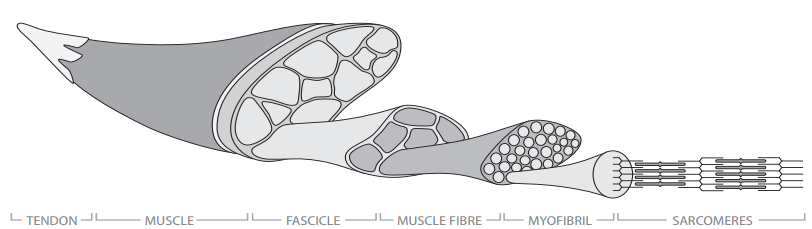
\includegraphics[width=0.7\linewidth]{images/muscle_struct}
	\caption[Строение мышцы]{Строение мышцы}
	\label{fig:musclestruct}
\end{figure}

\par Мышечное брюшко окружено плотным и прочным покровом, который называется фасцией. Внутри же содержаться различной толщины пучки мышечных волокон, каждое из которых образованно параллельными миофибриллами. Миофибрилы являются нитевидными образованиями, состоящими из саркомеров. 
\par Все соединительные образования мышцы с мышечного брюшка переходят на сухожильные концы. Они состоят из плотной волокнистой соединительной ткани, коллагеновые волокна которой лежат между мышечными волокнами, плотно соединяясь с их сарколеммой (оболочкой мышечных волокон).
\par Значительное влияние на работу мышц оказывает направление их волокон. По этому признаку выделяют: мышцы с параллельными, поперечными и косыми волокнами. Косые в свою очередь делятся на одноперистые, если присоединяются к сухожилию с одной стороны, и двуперистые, если с двух сторон. Данные особенности в строении определяют то, насколько подвижными являются мышцы и какую силу они могут производить.
\par При сокращении центральная нервная система подаёт сигнал в мышцы, в результате которого нити саркомеров скользят друг вокруг друга, что приводит к укорачиванию саркомера~\cite{muscle_03}. Скольжение нитей вызывает мышечное напряжение, что является основным вкладом саркомера, так как именно это действие даёт мышцам их физическую силу. 
\par Задачей программы является представление визуальной модели мышц, которая позволила бы наблюдать за процессом их сокращения, благодаря чему было бы проще изучить их строение и основные принципы работы.
\par Следует отметить, что существуют приложения, позволяющие изучать строение мышц. Некоторые из них также моделируют внутренние органы, однако в них возможно наблюдать только мышцы только в статическом положении. Это отличает эти приложения от разрабатываемого мной, которое позволит изучать процесс сокращения.
 \begin{figure}[h]
 	\centering
 	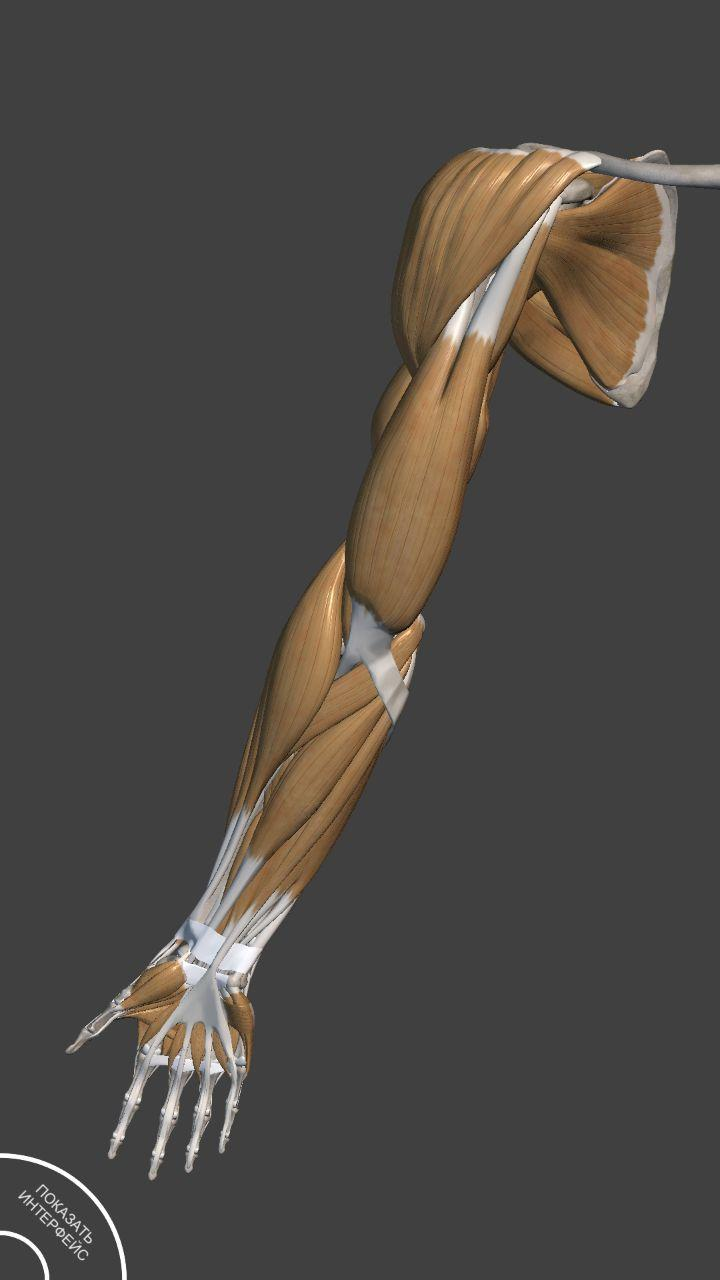
\includegraphics[width=0.3\linewidth]{images/ex1}\quad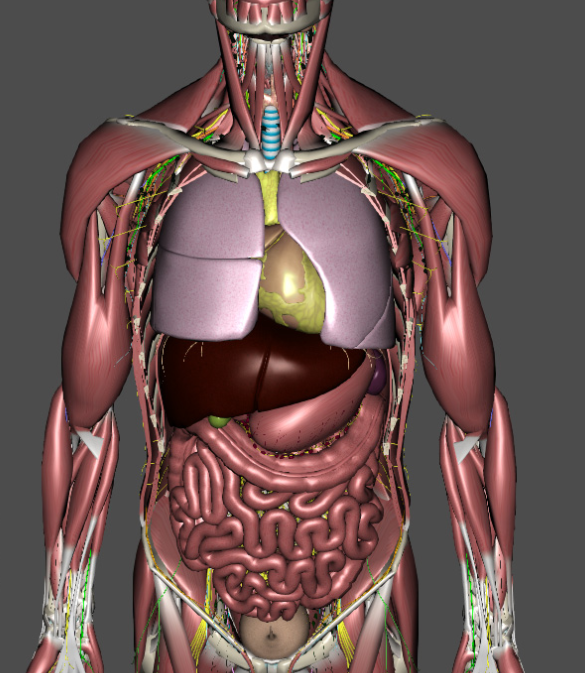
\includegraphics[width=0.3\linewidth]{images/ex2}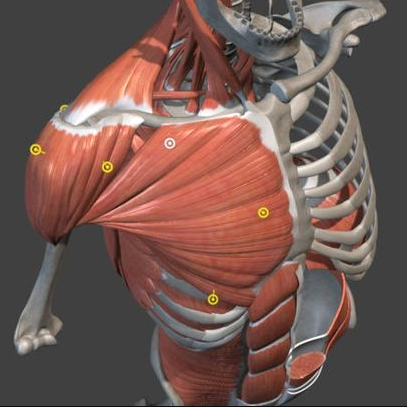
\includegraphics[width=0.3\linewidth]{images/ex3}
 	\caption{Примеры анатомических атласов}
 	\label{fig:ex1}
 \end{figure} 

\newpage
\section{Способы моделирования мышечных сокращений}
\label{sec:muscle_meth}
Существуют различные способы представления мышечных сокращений. В зависимости от принципов, лежащих в основе каждого из методов, их можно разделить на: геометрически-основанные и физически-основанные~\cite{diff_methods}. В геометрически-основанных подходах большее внимание уделяется анимации расширения и укорачивания, в то время как физический аспект сокращения не учитывается. Они успешно моделируют простые мышцы, но им недостаёт реализма в физиологическом или биомеханическом аспектах. В противовес к таким подходам ставятся физически-обоснованные подходы, в которых рассматриваются сложные проблемы, включающие в себя динамику мышц и свойства тканей. Чтобы смоделировать физически-корректную модель мышц решают две проблемы: определение силы сокращения и представление изменения мышечной геометрии.

\subsection{Использование деформируемых эллипсоидов для аппроксимации мышц}
\label{subsec:elypsoids}
Идея данного метода заключается в использовании параметрических эллипсоидов в качестве базовых примитивов для моделирования мышц. Три главные оси отрегулированы так, чтобы представлять выпуклость мышечного брюшка, в то время как объём сохраняется за счёт использования определённых соотношений между этими тремя осями~\cite{scheepers97}. Чтобы симулировать изометрические сокращения мышц, вводится параметр напряжённости t, в связи с чем соотношение шириной и высотой эллипсоида рассчитывается по формуле:
\begin{equation}\label{r_eq}
r = (1 - t)r_{n} + ktr_{n} = (1 - t + kt)r_{n}
\end{equation}
где k - параметр контроля напряжённости, который регулирует, насколько выпукла мышца, $r_{n} = \frac{a_{n}}{b_{n}}$ - соотношение ширины к высоте в расслабленном состоянии. 
\par Для представления более сложных форм могут использоваться сразу несколько эллипсоидов, расположенных на определённой кривой, или же прямой путь между концами мышцы может быть заменён кривой Безье, представляющей направление силы, и эллипсоидами разных размеров, расположенных вдоль этой кривой~\cite{scheepers97}

\subsection{Обобщённая цилиндрическая модель}
\label{subsec:cylinder}
Аналогичным подходом является представление мышц, основанное на деформируемых цилиндрах. Ось цилиндра - кривая, вдоль которой расположены эллиптические срезы. Именно на их основе строится полигональный меш~\cite{Wilhelms97}. Подразумевается, что каждый радиус, позиция и наклон каждого эллипса могут быть изменены, что позволяет формировать мышцы сложной формы.
\par При сокращении ширина и толщина внутренних срезов увеличивается в соотношении $\sqrt{l_{n} / l}$, где $l_{n}$ - длина в расслабленном состоянии, а $l$ - текущая длина. За счёт этого поперечная область расширяется, если мышцы становятся короче, и сужается, если удлиняются.
\par Другим способом является задание мышцы, используя модифицированный обобщенный цилиндр, определяемый с помощью кривой толщины $C_{T}(t)$ вдоль кривой наклона $C_{S}(t)$~\cite{ramos}. $C_{S}(t)$ это трёхмерный сплайн, представляющий профиль мышцы. Он определяется двумя точками - источником O и целью I. $C_{T}(t)$ - одномерная функция, представляющая толщину мышцы от t. Срез мышцы в t определяется эллипсом, расположенным вдоль $C_{S}(t)$, толщина которого получена из $C_{T}(t)$. Чтобы избежать пересечения секций и упростить сохранение объёма, поперечное сечение всегда расположено перпендикулярно линии действия, лежащей на главной оси мышечной формы.

\subsection{Mass-spring System}
\label{subsec:MSS}
Объект моделируется набором точечных масс, связанных между собой невесомыми пружинами. Такая модель может быть расширена при добавлении различных типов сил, применяемых к пружине, таких как угловую или силу сжатия. Линии, называемые линиями действия, используются для вычисления силы, прилагаемой к костям при сокращении~\cite{nedel}. В зависимости от формы и сложности их строения, мышцы могут быть представлены одной или несколькими линиями действия, кроме того каждая линия может быть полилинией.
\par Такой подход позволяет разделить модель на 2 уровня: линию действия, задаваемую точками начала и конца, и форму мышцы. Важной частью формирования данной модели является установление соответствия между точками массы и формой мышц. Для этого каждая точка должна быть расположена между двумя соседними в горизонтальном и двумя другими в вертикальном смысле. Чтобы модель мышц удовлетворяла этим требованием, необходимо несколько изменять форму ее меша. Из-за чего происходят потери в качестве. Кроме того, такой подход применим только к мышцам, обладающим вытянутой формой~\cite{nedel}.
\par Преимуществом модели, использующей точки масс является возможность рассчитать силу сокращения для каждой точки, используя формулу, в которой сила упругости, действующая на неё определяется суммой сил, с которыми пружины, связывающие ее с 4 соседями, притягиваются:
\begin{equation}\label{mss_01}
f_{result}(x_{i})=f_{elasticity}(x_{i})+f_{curvuture}(x_{i})+f_{constraints}(x_{i})
\end{equation}
\begin{equation}\label{mss_02}
f_{elasticity}=\sum_{j=0}^{3}f_{spring_{j}}(x_{i})=\sum_{j=0}^{3}-ks(x_{i}-x_{rest})
\end{equation}
где $ks$ - коэффициент упругости пружины, $x_{i}$ - экстремум её колебания, $x_{rest}$ - расслабленное положение этого экстремума. Для формирования искривлённости мышцы вводятся дополнительные пружины, соединяющие не соседние точки.

\subsection{Метод конечных элементов}
\label{subsec:FEM}
В основе этого метода лежит разбиение тела на набор конечных элементов, например гексаэдров или тетраэдров. Перемещения и положения в элементе аппроксимированы с помощью интерполяционных функций:
\begin{equation}\label{eq:FEM}
\Phi(x)\approx\sum_{i}h_{i}(x)\Phi_{i}
\end{equation}
где $h_{i}$ - интерполяционная функция для элемента, содержащего x и $\Phi_{i}$ - скалярный вес, сопоставленный с $h_{i}$ Такой подход часто применяется для представления твёрдых упругих тел. \par Одним из способов применения метода конечных элементов является модель, в которой кроме полигонального представления мышц, применяются двадцати-вершинные блоки, являющиеся "двигателем" модели~\cite{chen}. После чего для сетки каждого блока формируются динамические уравнения равновесия. Механическая модель мышц используется для приложения сил к вершинам блоков,  после чего их форма динамически меняется, что в свою очередь оказывает влияние на полигоны. Для двадцати-вершинного блока уравнение равновесия имеет вид:
\begin{equation}\label{key}
M\ddot{u}+C\dot{u}+Ku=R(t)
\end{equation}
Для тела, имеющего n узловых точек, u - это вектор размерности 3n, отображающий расположение вершин, M, C и K матрицы размерности 3n*3n, описывающие массу, затухание и жёсткость между точками внутри тела, и R - это вектор сил, прилагаемых к каждой вершине, размерностью 3n.
\par Чтобы симулировать мышечное сокращение, в вершинах добавляются генераторы силы, которые действуют вдоль продольного направления мышц. В двадцати-вершинном блоке расположено 8 таких генераторов.

\subsection{Метод конечных объёмов}
\label{subsec:FVM}
Аналогично предыдущему методу метод конечных объёмов разбивает модель на множество элементов. Однако для расчёта прилагаемых сил объёмные интегралы трансформируют в интегралы по площади, используя формулу Гаусса-Остроградского. Эти условия затем расцениваются как потоки на поверхности каждого конечного объёма. Эта модель используется для представления деформации скелетных мышц, и считается, что она более производительна и обладает меньшим потреблением памяти, чем метод конечных элементов~\cite{teran}.
\paragraph{Вывод} было решено использовать модель, использующую деформируемые эллипсоиды для аппроксимации мышцы, так как она позволяет визуализировать мышцы различных форм и размеров, учитывая изометрическое сокращение мышц.

\section{Выбор методов моделирования}
\label{sec:model_meth}
Выделяют три основных типа моделей: каркасные, граничные и сплошные~\cite{nikulin}. Каркасная конструкция в виде проволочной сетки является простейшим способом передачи формы объёмного тела. Проволочные модели дают возможность быстро визуализировать низко детализированные объекты.
\par Граничная модель представляет объект системой элементов, создающих его границы. Для задания границ могут использоваться аналитическая и векторная полигональная модели~\cite{porev}. Первая - это такая модель, в которой для описания поверхности используются математические формулы. Например в виде функций двух аргументов $ z = f(x, y)$ или уравнением $F(x, y, z) = 0$.
\par Преимущества параметрического описания - легко описывать поверхности, которые отвечают неоднозначным функциям, лёгкость процедуры расчёта координат каждой точки поверхности, нормали; небольшой объём информации для описания достаточно сложных форм.
\par К недостаткам относятся следующие: невозможность в большинстве случаев применения данной формы непосредственно для построения изображения; некоторые сложные формулы описания могут медленно вычисляться на компьютере~\cite{porev}.
\par Другим способом задания пространственных объектов является векторная полигональная модель. Ее основными элементами являются: вершины, отрезки прямых, полилинии, полигоны, полигональные поверхности. Векторная полигональная модель считается наиболее распространённой в современных системах трёхмерной графики. Положительными чертами векторной полигональной модели являются:
\begin{itemize}
	\item удобство масштабирования объектов, диапазон которого определяется точностью аппроксимации;
	\item небольшой объём данных для описания простых поверхностей, аппроксимируемых плоскими гранями;
	\item необходимость вычислять только координаты вершин при преобразованиях систем координат или перемещении объектов.
\end{itemize}
Недостатки:
\begin{itemize}
	\item аппроксимация плоскими гранями приводит к погрешности моделирования;
	\item сложные алгоритмы выполнения топологических операций, таких, например, как разрезы.
\end{itemize}
\par Сплошная модель включает в объект как граничные, так и внутренние точки. Это позволяет представлять сложный объект в виде композиции простых составляющих - кубов, сфер, конус и т.д. Простейшая декомпозиция заключается в разбиении пространства на кубические или сферические ячейки, называемые вокселами, и установления состояния каждой ячейки - свободна она или занята объёмом тела. Преимущества такой модели:
\begin{itemize}
	\item позволяет достаточно просто описывать сложные объекты и сцены;
	\item простое выполнение топологических операций над отдельными объектами и сценой в целом.
\end{itemize}
Недостатки:
\begin{itemize}
	\item большое количество информации, необходимой для представления объемных данных;
	\item значительные затраты памяти ограничивают разрешающую способность, точность моделирования;
	\item при увеличении или уменьшении изображения возникают проблемы, например при увеличении ухудшается разрешающая способность.
\end{itemize}
\paragraph{Вывод:} выбирая между методами моделирования, было решено использовать полигональный, так как он является более экономичным по памяти, чем воксели. Кроме того, такое представление позволяет легко изменять форму модели, что положительно влияет на производительность, при анимации сокращения мышц. 

\section{Выбор метода морфинга}
\label{sec:morph}
Морфинг - это интерполяционная техника, используемая для создания плавной трансформации одного изображения в другое~\cite{volume_morph}. Для изображений, сгенерированных на основе трёхмерных моделей, существует альтернатива морфингу самого изображения: трёхмерный морфинг, который формирует промежуточные модели на основе заданных, они затем используются, чтобы произвести последовательность изображений. Преимуществами такого подхода являются:
\begin{itemize}
	\item промежуточные формы не зависят от точки обзора и свойств освещения;
	\item двумерным техникам не достаёт информации о пространственной конфигурации модели, в связи с чем они не могут корректно обрабатывать изменения в освещении и видимости~\cite{volume_morph}.
\end{itemize}
Трёхмерные техники могут применяться к моделям, заданным объёмами или гранично описанными -- мешами. Меш $M$ можно описать парой $(K, V)$, где $K$ -- это набор, отображающий связь вершин, рёбер и граней и $V = (v_{1},\dots,v_{n})$ -- описывает геометрическое положение вершин в $R^{d}$~\cite{alexa}. Обычно, морфинг применяются к двум заданным мешам $M_{0}=(K_{0},V_{0})$ и $M_{1}=(K_{1},V_{1})$. Целью является построение группы мешей $M(t)=(K,V(t)),t\in[0,1]$, генерация ее обычно выполняется за три последовательных шага~\cite{alexa}:
\begin{enumerate}[1.]
	\item Поиск соответствия между мешами. А именно сопоставление вершин, лежащих в исходной фигуре, с вершинами целевой фигуры.
	\item Формирование новой, последовательной связности $K$ для каждой вершины на основе геометрических позиций $V(0), V(1)$. Традиционный подход к этой проблеме заключается в создании надмножества $K_{0}$ и $K_{1}$. Однако, в некоторых случаях ремешинг может быть полезен в случае, когда исходные меши обладают разными разрешениями.
	\item Создание путей $V(t),t\in]0,1[$ для вершин. Данный шаг обладает некоторыми ограничениям: в большинстве случаев не ожидается, что форма будет разрушаться или самопересекаться, и, как правило, ожидается, что пути будут гладкими. Самый простой способ, получить такие пути - это линейная интерполяция координат вершин. При заданном параметре $t$ координаты интерполированной формы вычисляются как:
	\begin{equation}
	V(t)=(1-t)V(0)+tV(1)
	\end{equation}
	Такая интерполяция даст хорошие результаты, если формы одинаково ориентированны и в некоторой степени похожи.
\end{enumerate}
\par Для определения, в какое положение должен перейти тот или иной полигон, можно использовать, например, методы ближайшего соседа и сортировки рёбер~\cite{morphing}. Идея метода ближайшего соседа заключается в поиске наименьшего расстояния между треугольниками, но вместо трёхмерного пути, который прошли бы центры этих рёбер при перемещении, рассматриваются возможные перестановки вершин и из них выбирается наименьшее. Так, для двух треугольников возможно 6 перестановок, но 3 из инвертирует нормаль к полигону, в связи с чем рассматриваются 3 оставшиеся, из них выбирается та, которая минимизирует путь, необходимый для перемещения из одного набора вершин в другой. Однако такой метод не гарантирует, что все сопоставления будут уникальными.
\par Другой метод - сортировка рёбер, в нем каждый треугольник рассматривается как узел а каждое сопоставление между двумя треугольниками - ребро. И поскольку определение соответствия выполняется между двумя множествами источников и целей, проблема сводится к формированию двудольного графа, который соединяет все вершины, и каждую только один раз. В таком случае алгоритм состоит из следующих шагов:
\begin{itemize}
	\item Сформировать полный взвешенный биграф, в котором вес - расстояние между двумя полигонами, как в методе ближайшего соседа.
	\item Упорядочить все ребра по весу.
	\item Для каждого ребра, в сортированном списке, если обе вершины свободны, то установить соответствие, иначе выбрать следующее.
\end{itemize}
В результате для каждого полигона будет однозначно установлен полигон, в который он должен перейти.

В случае, когда морфинг применяется к объёмно-заданной модели, проблема может быть сформирована так - даны два объёма S и T, необходимо произвести последовательность промежуточных объёмов, удовлетворяющим условиям реалистичности и плавности~\cite{volume_morph}. Создание этих состояний разбивается на два этапа:
\begin{itemize}
	\item Искривление - S и T искривляются, чтобы получить объёмы S' и T'. Для этого могут задаваться пары элементов, один элемент из исходного и один в результирующим объёмах. Необходимо задать несколько таких пар, которые определят общее соответствие между двумя объектами. Эти пары объектов взаимодействуют как магниты, формирующие податливые объёмы~\cite{volume_morph}.
	\item Смешивание может выполняться перекрёстным растворением объёмов или же их двумерных изображений. Под смешиванием объемов подразумевается интерполяция вокселей, из которых они состоят.
\end{itemize}
\paragraph{Вывод:} было решено использовать трёхмерный морфинг на основе мешей, что связано с ранее выбранным методом полигонального представления модели, так как это позволит получить плавную анимацию с учётом освещения и видимости. Кроме того, этот метод даст хорошие результаты, поскольку форма мышц при сокращении не слишком сильно изменяется.

\section{Анализ методов удаления невидимых граней}
\label{sec:inv_edge}

\paragraph{Алгоритм Роберста} работает в объектном пространстве с выпуклыми телами. Если имеются невыпуклые тела, то их сначала необходимо разбить на выпуклые~\cite{rogers}. В алгоритме в первую очередь удаляются те ребра и грани, которые экранируются самим телом, затем каждое из видимых рёбер каждого тела сравнивается с каждым из оставшихся тел для определения того, какая его часть или части экранируются другими телами.
\par Недостатком алгоритма Робертса является то, что теоретически его вычислительная ёмкость растёт как квадрат числа объектов. Однако существуют модификации алгоритма с использованием приоритетной сортировки вдоль оси z и простых габаритных или минимаксных тестов~\cite{rogers}, которые позволяют свести вычислительную сложность к почти линейной зависимости от числа объектов.

\paragraph{Алгоритм Варнока} работает в пространстве изображений. Идея алгоритма заключается в том, что рассматривается окно и решается вопрос о том, пусто оно или нет его содержимое достаточно просто для визуализации~\cite{rogers}. В противном случае окно разбивается на более маленькие области, для которых снова решается этот вопрос. Предполагается, что если размер окна в результате его разбиения стал совпадать с одним пикселем, но при этом оно содержит не один многоугольник, то необходимо визуализировать тот из них, у которого максимальное значение координаты Z.
\par Недостатком алгоритма может являться необходимость проведения большого количества разбиений, что негативно скажется на временной эффективности.

\paragraph{Алгоритм, использующий Z-буфер} является одним из простейших алгоритмов удаления невидимых поверхностей~\cite{rogers}. Он работает в пространстве изображения. 
\par Суть алгоритма заключается в использовании Z-буфера, в котором запоминается координата z каждого видимого пикселя, в то время как буфер кадра используется для запоминания атрибутов каждого пикселя. В процессе работы глубина очередного пикселя сравнивается с глубиной, находящейся в Z-буфере, и в результате сравнения либо заносится в этот буфер, или никаких действий не производится.
\par Преимуществом данного алгоритма является его простота. Кроме того, он позволяет работать со сценами любой сложности, делая тривиальной визуализацию пересечений сложных поверхностей. Алгоритм обладает не более чем линейной вычислительной трудоёмкостью.
\par Недостатком же алгоритма является необходимость хранить Z-буфер, что увеличивает затраты по памяти, однако для современных компьютеров они являются незначительными~\cite{rogers}.

\paragraph{Алгоритм трассировки лучей} - метод грубой силы~\cite{rogers}. Главной идеей данного метода является запуск луча для каждого пикселя картинной плоскости, для каждого луча происходит проверка на пересечение с каждым из объектов сцены, после чего пересечения упорядочиваются по глубине. Пересечение с максимальным значением z представляет видимую поверхность для данного пикселя.
\par К достоинствам алгоритма можно отнести то, что вычислительная сложность метода линейно зависит от сложности сцены. В результате выполнения алгоритма получается очень реалистичное изображение. А также метод даёт возможность создания гладких объектов без аппроксимации их примитивами.
\par Однако для получения такого изображения необходимо создать огромное количество лучей, проходящих через сцену, и необходимость нахождения пересечения с каждым из объектов, что негативно сказывается на скорости работы программы.
\par Чтобы уменьшить количество искомых пересечений производится поиск пересечения луча с объёмной оболочкой рассматриваемого объекта. Если оно не найдено, то нет необходимости в поиске пересечения с объектом. В качестве оболочки можно применять параллелепипед или сферу.
\paragraph{Вывод:} было решено использовать алгоритм, использующий Z-буфер, поскольку его реализация проще, чем у других алгоритмов, в то время как его вычислительная трудоёмкость сохраняется линейной. И, как уже было отмечено раньше, затраты памяти, связанные с хранением Z-буфера, больше, чем у других алгоритмов, они всё же незначительны для современных вычислительных машин.


\section{Анализ моделей освещения}
\label{sec:light}
Простая модель освещения ограничивается отображением света, исходящего от явных точечных источников. В ней не учитываются взаимодействия объектов сцены между собой, но учитывается диффузное отражение света. Интенсивность света, отражённого предметом вычисляется по формуле:
\begin{equation}\label{lambert}
I = I_{a}k_{a} + I_{l}k_{d}\cos \theta \qquad 0\leq\theta\leq\pi/2
\end{equation}
Глобальная модель описывает освещение, учитывая взаимное влияние объектов сцены. Она рассматривает многократное отражение и преломление света, рассеянное освещение. Для этого отслеживается путь луча до тех пор, пока он не покинет сцену или его энергия не станет достаточно малой, чтобы не учитывать ее. Глобальная модель освещения позволяет получить более реалистичное изображение.
\paragraph{Вывод:} для визуализации мышц можно пренебречь преломлением и бликами, так что было решено использовать простую модель освещения, используя формулу Ламберта. Кроме того использование такой модели позволит выиграть в производительности.

\section{Анализ методов закраски}
\label{sec:color}
\paragraph{Метод простой закраски-} его идея заключается в том, что для каждой грани объекта находится вектор нормали, с помощью которого в соответствии с выбранной моделью освещения вычисляется значение интенсивности, с которой закрашивается вся грань.
\par Метод простой закраски обладает наилучшим быстродействием, однако все пиксели грани обладают одинаковой интенсивностью, в связи с чем сцена может выглядеть нереалистично.

\paragraph{Метод Гуро} позволяет получить более сглаженное изображение, чем простая закраска. Такой результат получается за счёт билинейной интерполяции интенсивностей в пределах одной сканирующей строки.
\par Недостатками метода Гуро является появления полос Маха в связи с тем, что такой метод интерполяции не обеспечивает непрерывности изменения интенсивности, а также то, что некоторые рёбра могут казаться сглаженными.

\paragraph{Метод Фонга} требует больших вычислительных затрат, чем закраска по Гуро. Идея такой закраски заключается в интерполировании вектора нормали вдоль сканирующей строки, который затем используется в модели освещения для расчёта интенсивности.

\paragraph{Вывод:} выбирая между методами закраски было решено использовать метод простой закраски, который является, самым быстрым из представленных, что позволит отображать анимацию более плавно.

\section{Вывод}
\label{sec:conc_analysis}
В данном разделе была рассмотрена предметная область, аналоги разрабатываемому приложению, основные алгоритмы, необходимые для создания реалистичного изображения визуализации мышечных сокращений. Из них были выбраны:
\begin{itemize}
	\item использование деформируемых эллипсоидов для аппроксимации мышц;
	\item полигональный метод моделирования;
	\item трёхмерный морфинг на основе мешей;
	\item алгоритм Z-буфера для удаления невидимых граней;
	\item простая модель освещения.
\end{itemize}